\begin{titlepage}
\definecolor{verdeSuave}{HTML}{90EE90}


%Para cambiar el color busca el código HTML del color y definelo en el preambulo

\tikz[remember picture,overlay] \node[opacity=1.0, inner sep=0pt] at ([yshift=-2.5cm]current page.south){
\begin{tikzpicture}

    \begin{pgfonlayer}{background}
        \filldraw[RCimat] (-12,-8)--(-12,3)--(12,2)--(12,-8)--cycle; {BG};
     \end{pgfonlayer}

    \begin{pgfonlayer}{foreground}
    \filldraw[GCimat] (-12,0)--(-12,1)--(12,1)--(12,0)--cycle; {overlay};
    \end{pgfonlayer}

\end{tikzpicture}};


\par
\noindent
\Huge
\textbf{\bfseries\Huge Temas Selectos de Deep Learning: Análisis Multimodal para MIR | Tarea \#1}
\vspace{0.2cm}
\LARGE
\par
\noindent
Análisis Integral de Corpus en Español\\
\rule[0.3cm]{\linewidth}{2pt}


%%%%%%%%%%% Aquí va el código de los integrantes
\begin{minipage}{0.6\textwidth}
\begin{flushleft} \large
\Large{\emph{\textbf{César M. Aguirre Calzadilla}}}\\

%% Your name
\end{flushleft}
\end{minipage}
\vspace{0.5cm}
\begin{center}
    %{
\includegraphics[scale=0.3]{01_Portada/logo.jpeg}\hspace{2cm} 
    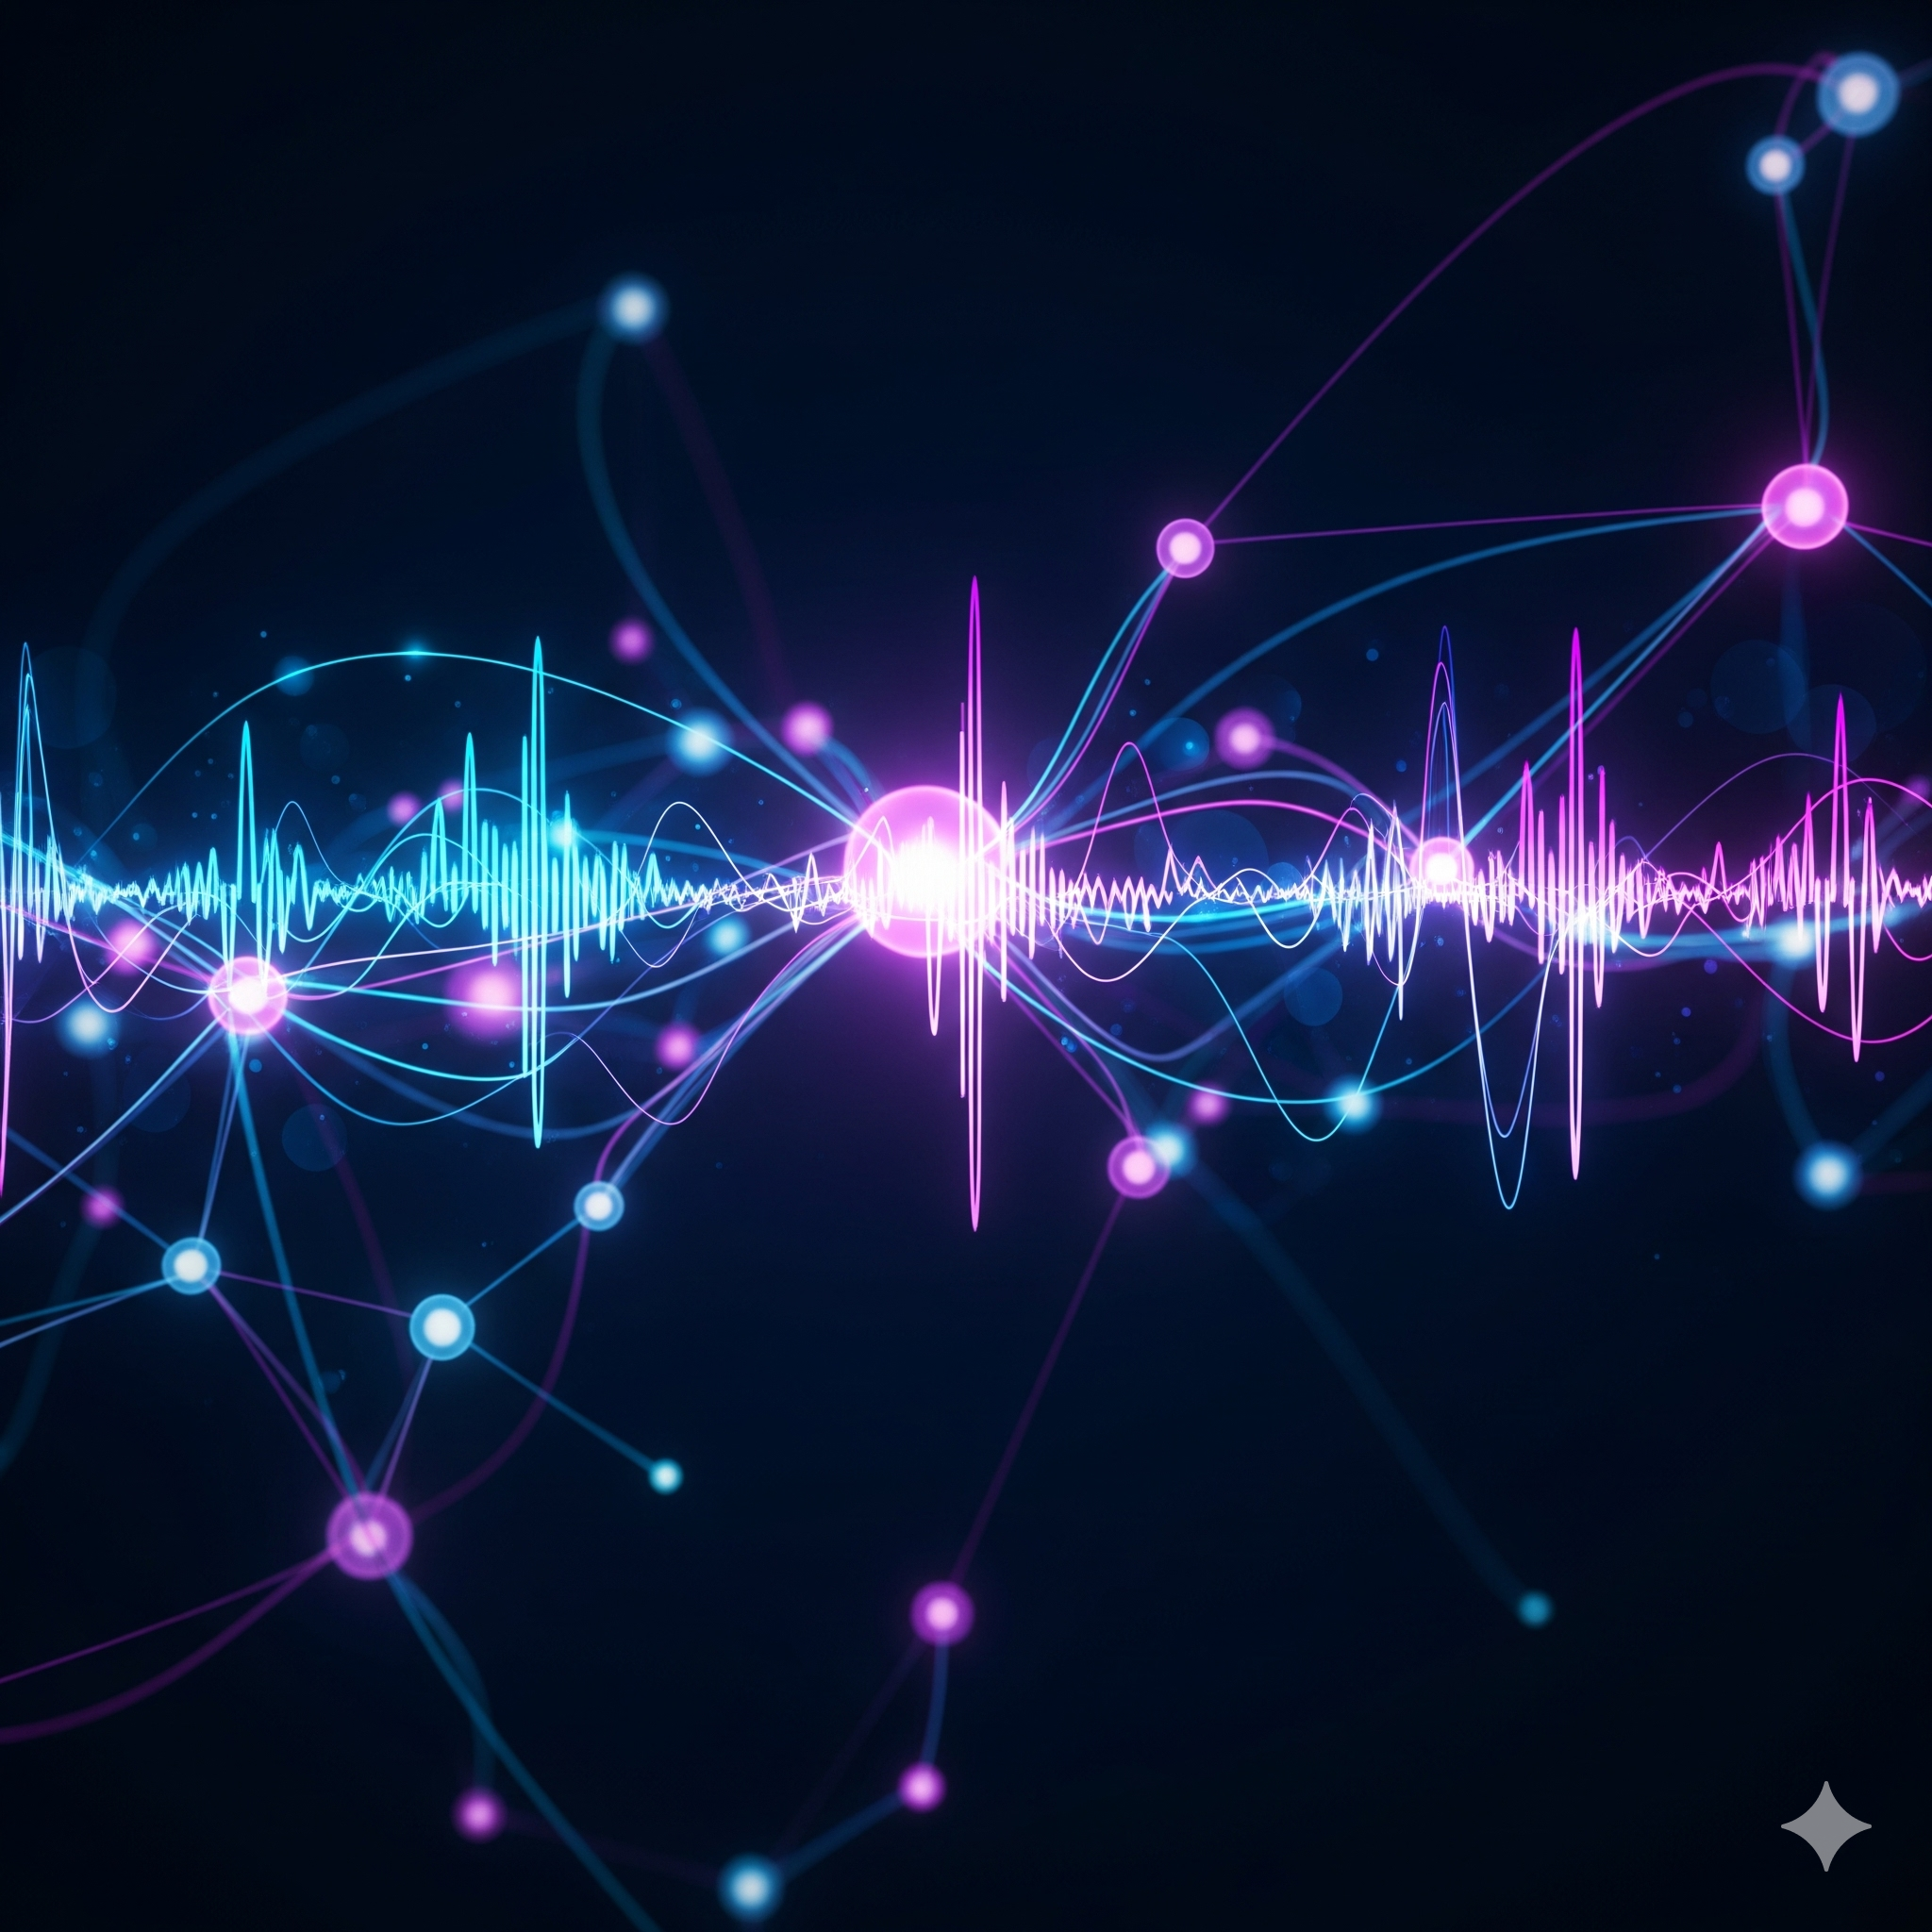
\includegraphics[scale=0.23]
    {Images/Portada.png}\par}
    \vspace{1cm}
    {\textit{\bfseries\huge Centro de Investigación en Matemáticas}\par}
    \vspace{0.5cm}
    {\large Maestría en Cómputo Estadístico\par}
    %\vspace{0.1cm}
    %{\large Ciencia de Datos\par}
\vspace{1cm}
\end{center}

\begin{center} \large
\Large{\emph{\textbf{Catedráticos:}}}\\
\large{Dr. Victor Muñiz Sánchez\par}
%\large{Dr. Francisco Javier Hernández López\par}
\vspace{0.3cm}
\large \today
\end{center}
\vspace{1cm}



\end{titlepage}
